\subsubsection{Ekstraksi Data Smart Contracts dari Blockchain Ethereum}

\begin{figure}[ht]
	\centering
	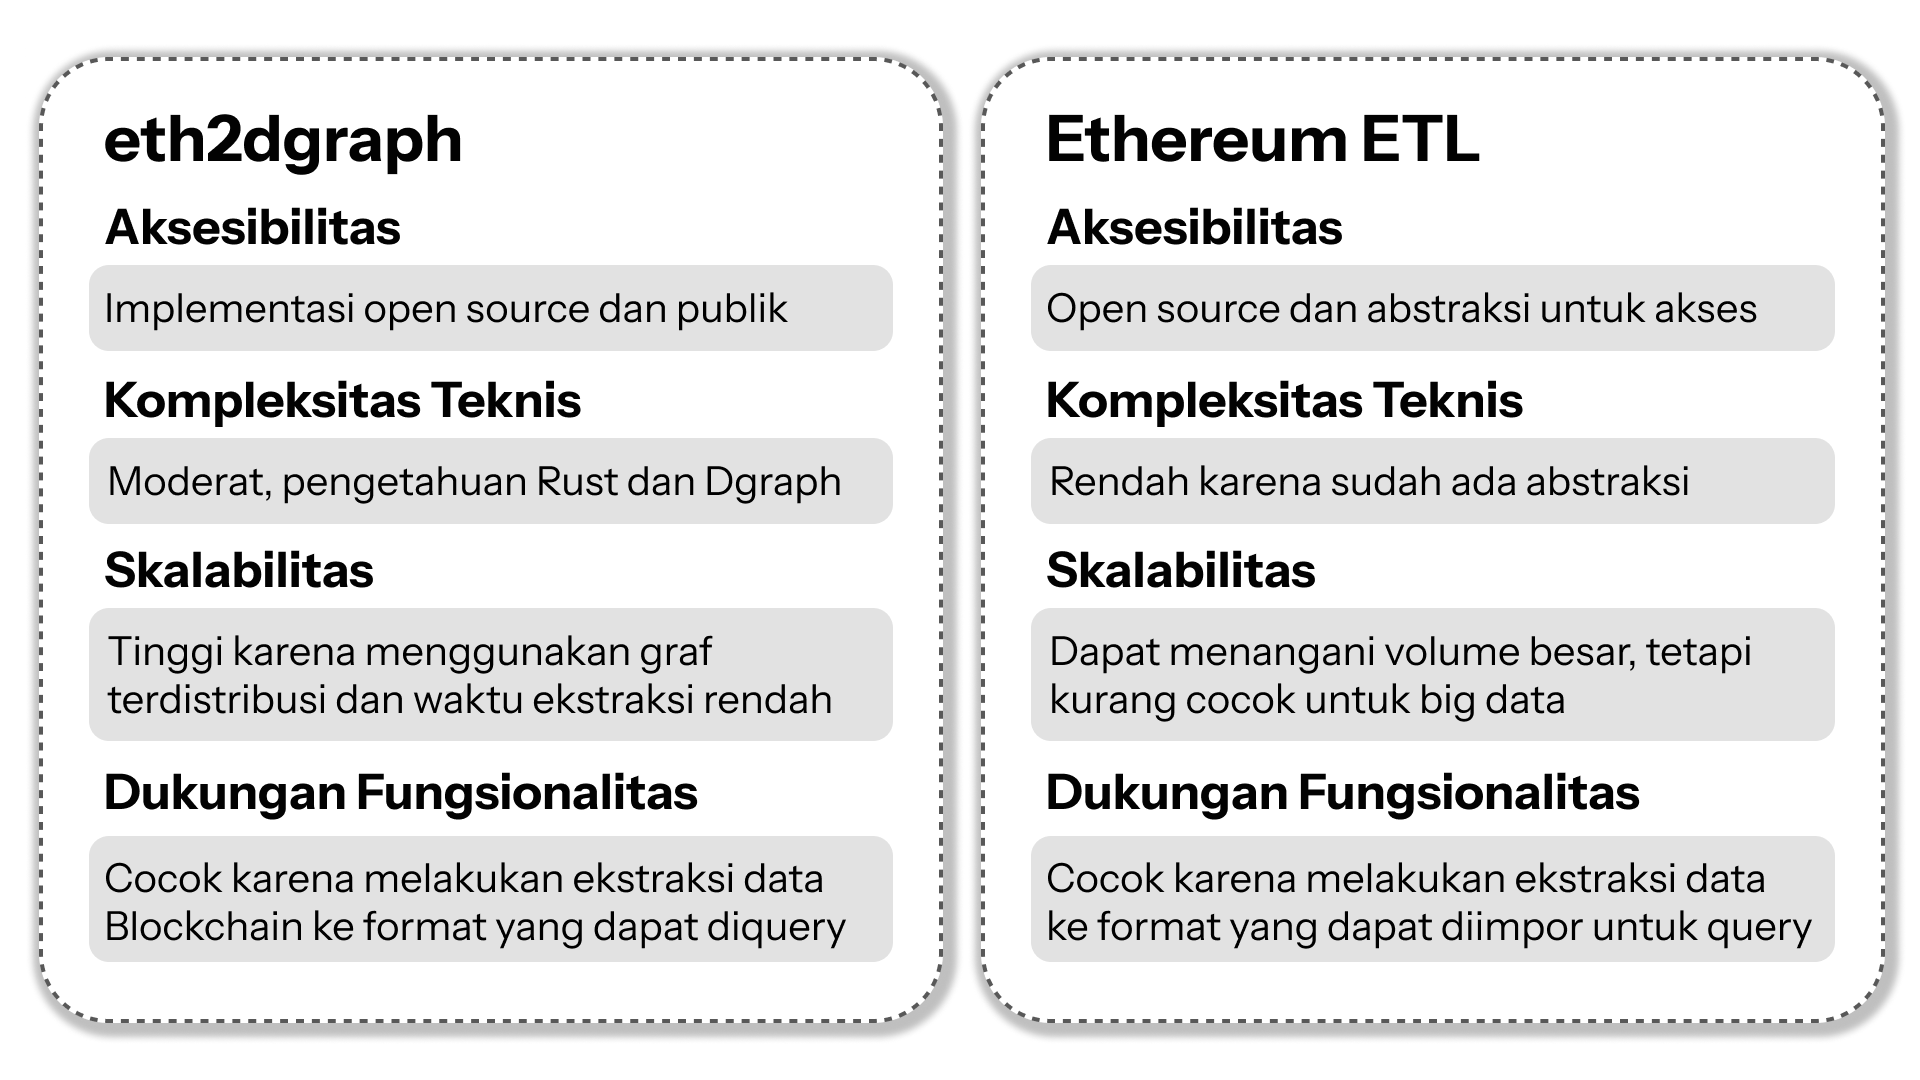
\includegraphics[width=0.7\textwidth]{resources/chapter-3/ekstraksi-1.png}
	\caption{Perbandingan alternatif ekstraksi data Smart Contracts dari Blockchain Ethereum}
	\label{image:perbandingan-ekstraksi-1}
\end{figure}

\begin{figure}[ht]
	\centering
	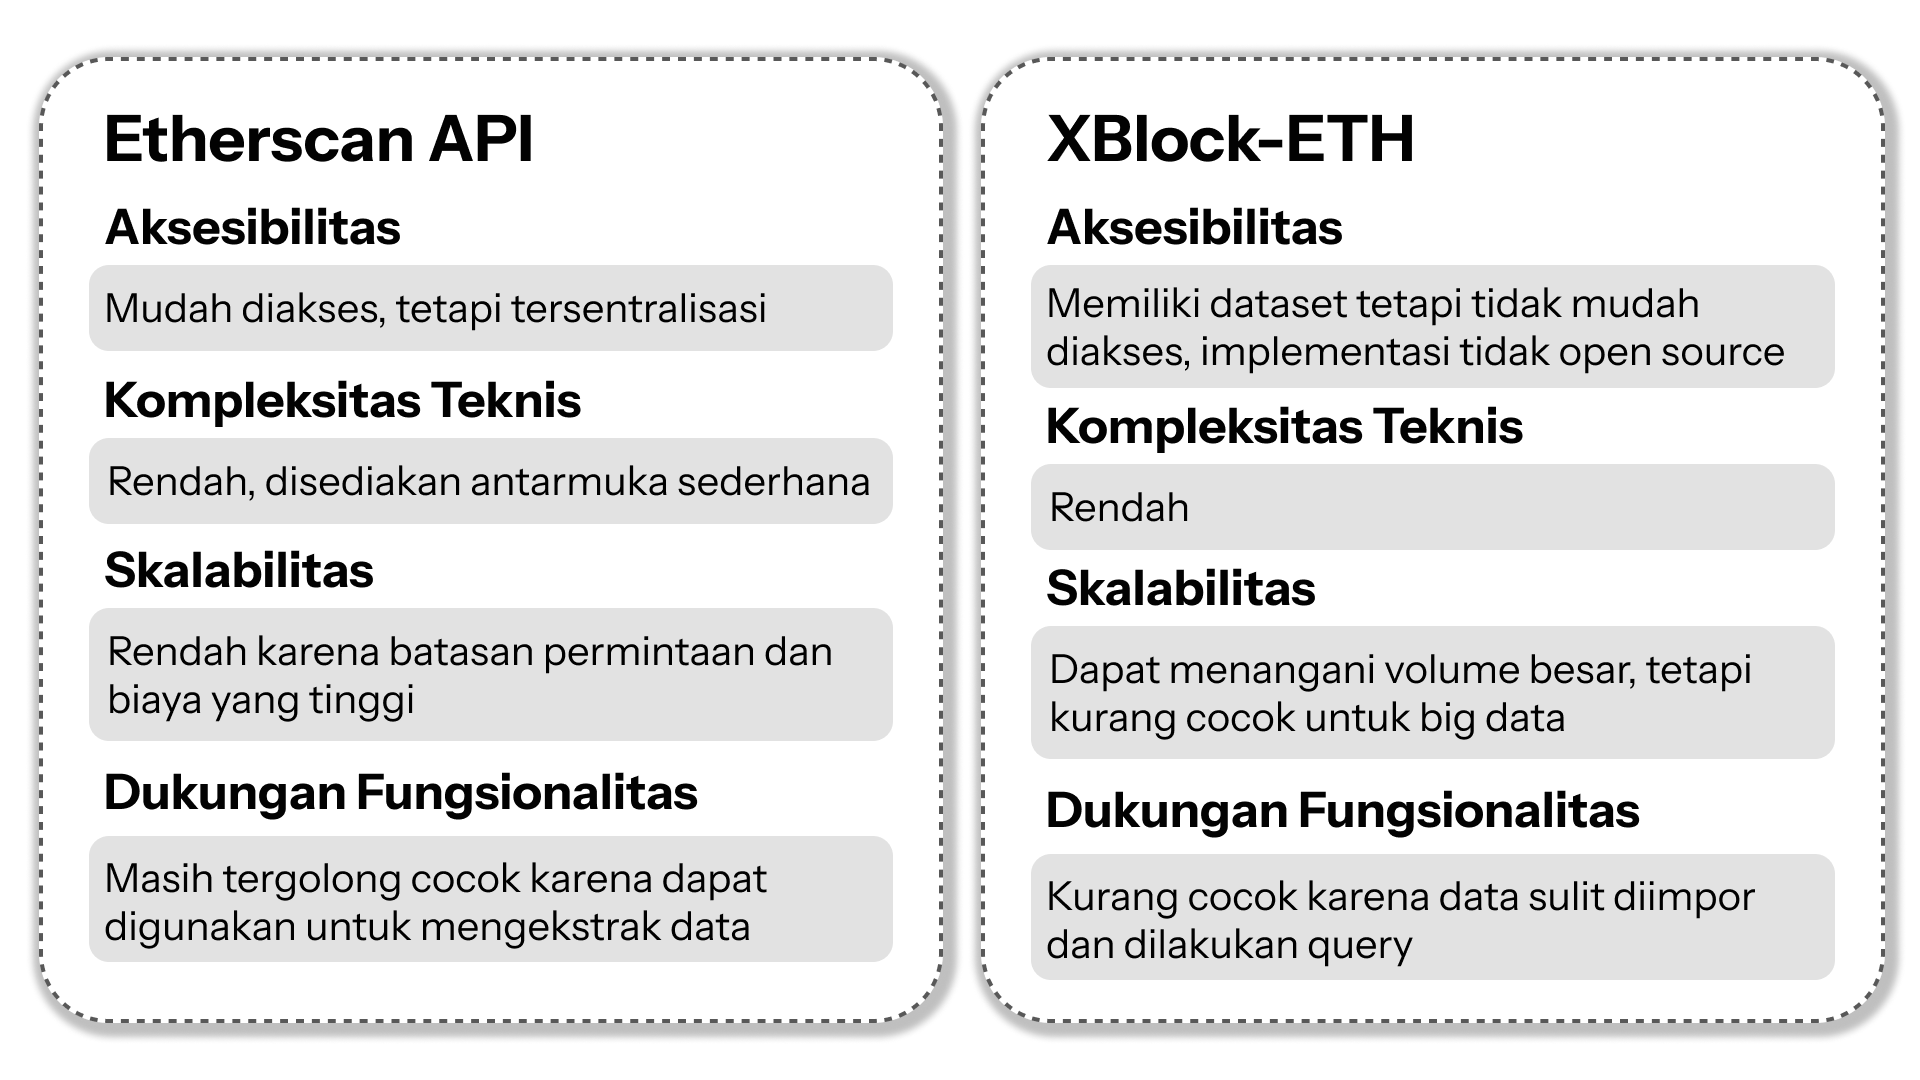
\includegraphics[width=0.7\textwidth]{resources/chapter-3/ekstraksi-2.png}
	\caption{Perbandingan alternatif ekstraksi data Smart Contracts dari Blockchain Ethereum}
	\label{image:perbandingan-ekstraksi-2}
\end{figure}

\begin{figure}[ht]
	\centering
	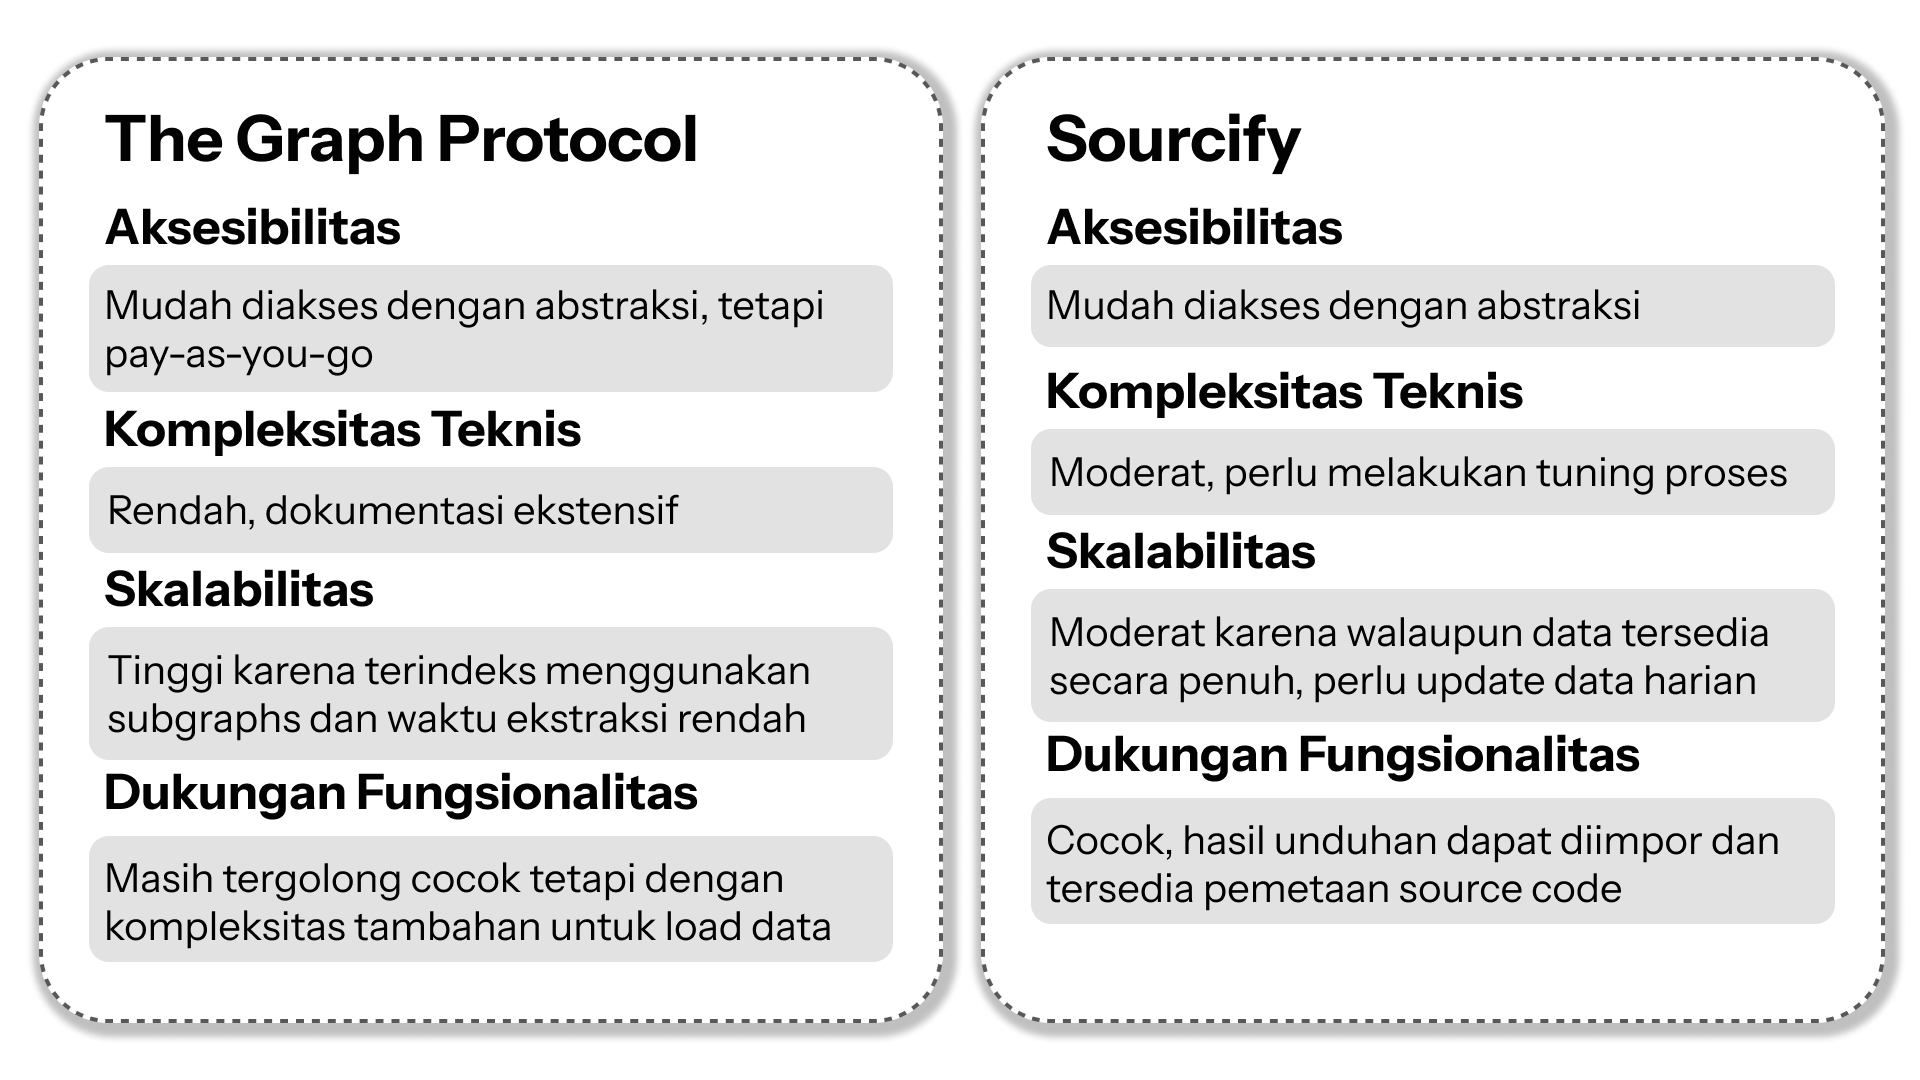
\includegraphics[width=0.7\textwidth]{resources/chapter-3/ekstraksi-3.png}
	\caption{Perbandingan alternatif ekstraksi data Smart Contracts dari Blockchain Ethereum}
	\label{image:perbandingan-ekstraksi-3}
\end{figure}

Seluruh data Blockchain Ethereum dapat diakses melalui Ethereum node yang terhubung ke jaringan Ethereum. Node ini dapat berupa node lokal yang di-\textit{hosting} sendiri atau layanan node publik seperti Infura, Alchemy, atau QuickNode. Terdapat beberapa riset yang dapat digunakan sebagai referensi atau dasar untuk melakukan ekstraksi data Smart Contracts dari Blockchain Ethereum, di antaranya adalah:

\begin{enumerate}
    \item \textbf{eth2dgraph} \parencite{aimar2023extraction}: Riset ini berfokus pada ekstraksi, \textit{indexing}, dan penyimpanan data Ethereum berbasis Distributed Graph. Keunggulannya adalah penggunaan ekstraksi ABI, bytecode, dan metadata yang dapat diubah menjadi format berbasis graf, serta implementasinya yang \textit{open source} dan \textit{public}. Untuk melakukan ekstraksi, dibutuhkan node Ethereum, baik yang dijalankan secara lokal maupun sebagai \textit{service}. Menggunakan Rust untuk kinerja tinggi dan Dgraph untuk skalabilitas, riset ini dapat melakukan query pada hubungan Smart Contracts di Ethereum. Kompleksitasnya moderat karena memerlukan pengetahuan dasar tentang Rust dan Dgraph, namun dapat diperluas untuk menambahkan aspek semantik. Skalabilitas dari hasil riset ini tinggi berkat kinerja Dgraph yang \textit{scalable}.
    
    \item \textbf{Ethereum ETL} \parencite{ethereum_etl}: Merupakan toolkit \textit{open source} berbasis Python untuk mengekstrak, mengonversi, dan memuat data blockchain Ethereum ke format yang mudah diolah (CSV, Parquet, BigQuery). Keunggulannya adalah kemudahan penggunaan dan dokumentasi yang baik, serta dukungan untuk berbagai jenis data seperti transaksi, blok, dan Smart Contracts. Secara kompleksitas, Ethereum ETL tergolong rendah karena menyediakan abstraksi layer ETL. Meskipun dukungan fungsional dari Ethereum ETL baik, terdapat beberapa kelemahan dari Ethereum ETL, yaitu tidak memiliki ekstraksi data ABI, membutuhkan waktu yang lama untuk melakukan ekstraksi data, dan diperlukannya beberapa operasi untuk mendapatkan data Smart Contracts. Secara skalabilitas, Ethereum ETL dapat menangani volume data besar dengan baik, namun mengeluarkan format data yang hanya cocok untuk basis data relasional, sehingga tidak cocok untuk sistem big data. 
    
    \item \textbf{Etherscan API} \parencite{etherscan2024}: Etherscan adalah salah satu penjelajah blok Ethereum yang paling populer. Menyediakan API yang memungkinkan pengguna untuk mengakses data Smart Contracts, transaksi, dan informasi lainnya dari Blockchain Ethereum. API ini dapat digunakan untuk mengekstrak data Smart Contracts secara langsung dari Etherscan, yang merupakan sumber data yang terpercaya dan terupdate. Secara aksesibilitas, Etherscan API mudah digunakan. Namun, data yang diekstrak dan di-\textit{indexing} berasal sepenuhnya dari Etherscan, sehingga pengguna perlu mempercayai Etherscan sebagai sumber data, dengan kata lain, sumber data Etherscan tersentralisasi. Selain itu, Etherscan API juga memiliki batasan pada jumlah permintaan dan memiliki biaya penggunaan yang dapat menjadi kendala untuk ekstraksi data dengan skala besar. Secara kompleksitas, Etherscan API tergolong rendah karena menyediakan antarmuka yang sederhana untuk mengakses data. Namun, pengguna perlu memahami cara menggunakan API dan mengelola batasan permintaan.
    
    \item \textbf{XBlock-ETH} \parencite{zheng2020xblock}: XBlock-ETH adalah alat yang dirancang untuk mengekstrak data dari Blockchain Ethereum kepada format CSV. Selain itu, XBlock-ETH juga merilis dataset yang sudah diekstrak pada website XBlock (\url{https://xblock.pro/xblock-eth.html}). XBlock-ETH memiliki keunggulan untuk mendapatkan data tanpa menggunakan Ethereum node, tetapi data yang disimpan dalam bentuk CSV perlu dilakukan \textit{parsing} dan tidak mudah dilakukan query atau \textit{indexing}. Selain itu, XBlock-ETH juga tidak mudah diakses karena kode untuk melakukan ekstraksi data tidak bersifat \textit{open source}, sehingga tidak dapat melakukan replikasi ekstraksi data. Secara kompleksitas, XBlock-ETH tergolong rendah karena tidak memerlukan pengetahuan teknis yang mendalam untuk menggunakannya. Namun, pengguna perlu memahami cara melakukan \textit{parsing} data CSV yang dihasilkan. Dalam hal skalabilitas, XBlock-ETH dapat menangani volume data besar dengan baik, tetapi tidak cocok untuk sistem big data karena format CSV yang dihasilkan tidak efisien untuk penyimpanan dan pemrosesan data besar.
    
    \item \textbf{The Graph Protocol} \parencite{TheGraphDocs}: The Graph adalah protokol dan Network untuk membangun dan mengelola indeks data terdesentralisasi dari Blockchain Ethereum. Protokol ini memungkinkan pengguna untuk membuat indeks data yang dapat di-query dengan efisien menggunakan GraphQL. Keunggulannya adalah kemudahan penggunaan dengan kemampuan untuk melakukan query dengan cepat. Secara aksesibilitas, The Graph dapat dengan mudah digunakan dan terintegrasi dengan baik, tetapi perlu pembayaran sesuai dengan penggunaan (\textit{pay-as-you-go}), yang membuat ekstraksi data lebih mahal. Secara kompleksitas, The Graph tergolong rendah karena dokumentasi ekstensif dan juga infrastruktur yang baik. Secara dukungan fungsional, The Graph menghasilkan data dalam bentuk json, yang perlu dilakukan impor ulang ke format yang dipilih, yang tidak mudah dan membutuhkan waktu lama, tetapi mudah di-\textit{extend}.
\end{enumerate}

Secara singkat, kelima riset ini dapat disimpulkan dengan diagram-diagram pada gambar \ref{image:perbandingan-ekstraksi-1}, gambar \ref{image:perbandingan-ekstraksi-2}, dan gambar \ref{image:perbandingan-ekstraksi-3}.

\newpage

% Setelah melakukan analisis dari alternatif yang ada, diputuskan untuk menggunakan riset oleh \cite{aimar2023extraction}, karena memiliki implementasi yang \textit{open source}, yang mempermudah ekstraksi dan \textit{indexing} data menjadi Distributed Graph Database, yang memiliki skalabilitas yang baik untuk data yang banyak pada Blockchain Ethereum. eth2dgraph juga memiliki kemampuan ekstensibilitas yang baik dalam \textit{domain} yang lebih umum, sehingga lebih mudah diimplementasikan sebagai fondasi dari sistem keseluruhan.